\documentclass{beamer}
\usetheme{Warsaw}

\usepackage[utf8]{inputenc}
\usepackage{fancybox}
\usepackage{multimedia} 
\usepackage{subfig}
\usepackage{amsmath}

\usepackage[all]{xy}
\begin{document}


\title[Computergrafik] % (optional, only for long titles)
{Computergrafik

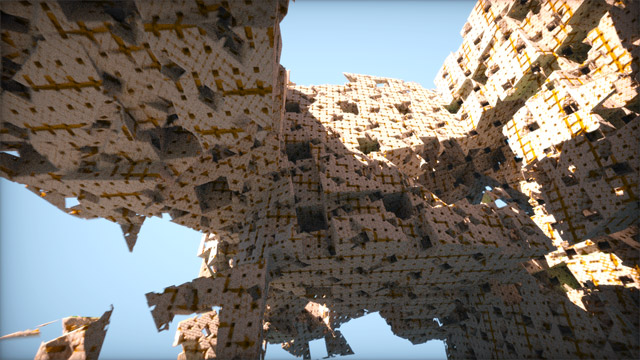
\includegraphics[scale=0.36]{images/cover}
}
\subtitle{}
\author[Dr. Johannes Riesterer] % (optional, for multiple authors)
{Dr.  rer. nat. Johannes Riesterer}

\date[KPT 2004] % (optional)
{}

\subject{Computergrafik}

\frame{\titlepage}


\begin{frame}
    \frametitle{Kameraprojektion}
\framesubtitle{}

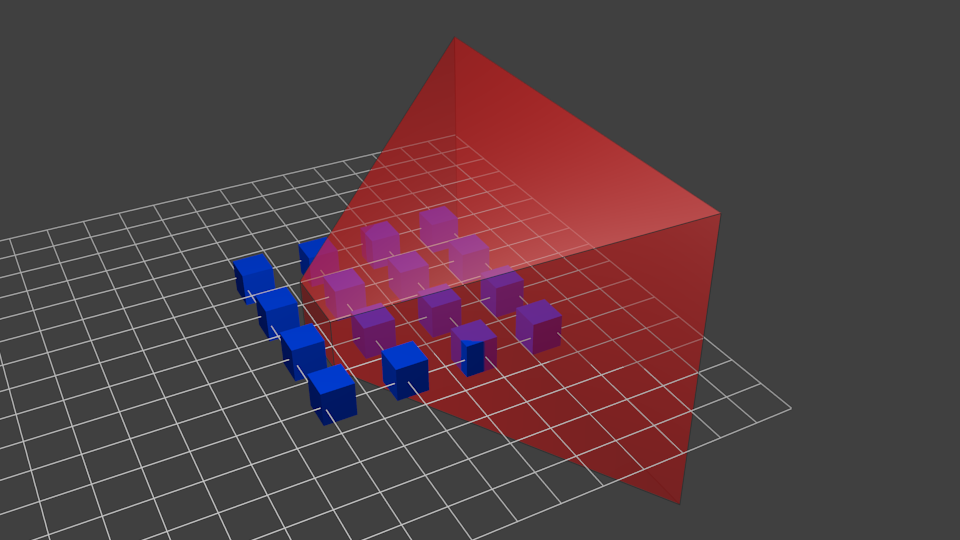
\includegraphics[scale=0.16]{images/nondeforme}
 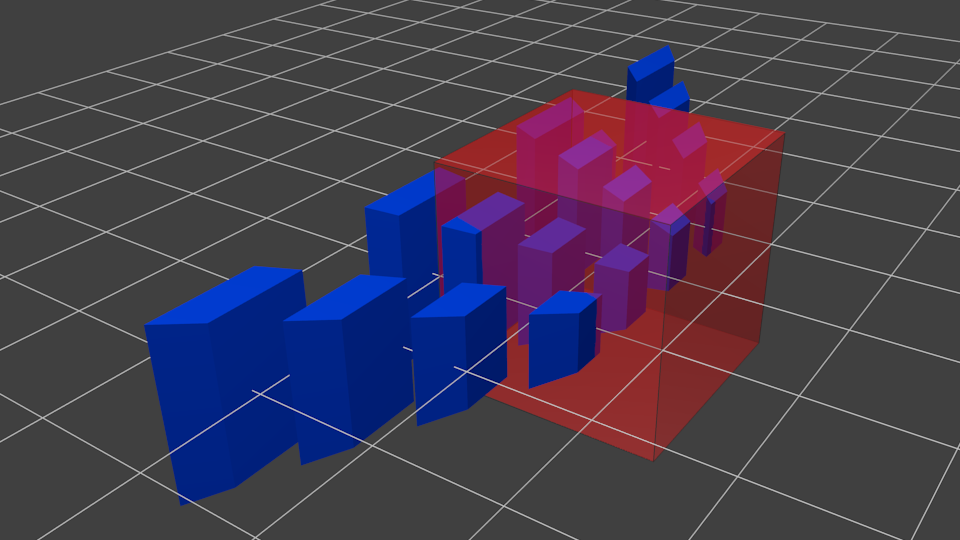
\includegraphics[scale=0.16]{images/deform}

\end{frame}


\begin{frame}
    \frametitle{ Shaderprogramm}
\framesubtitle{}
\begin{center}

\includegraphics[scale=0.26]{images/cgpipeline_grob}
\\
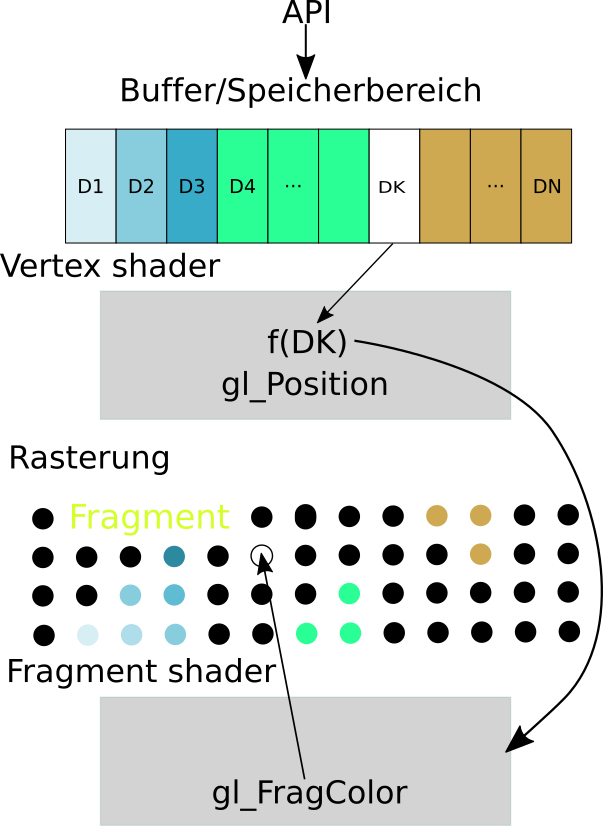
\includegraphics[scale=0.20]{images/Zeichnung_Shaderpipeline}

\end{center}
\end{frame}

\begin{frame}
    \frametitle{OpenGL Pipeline}
\framesubtitle{}
    \begin{block}{}
\begin{center}
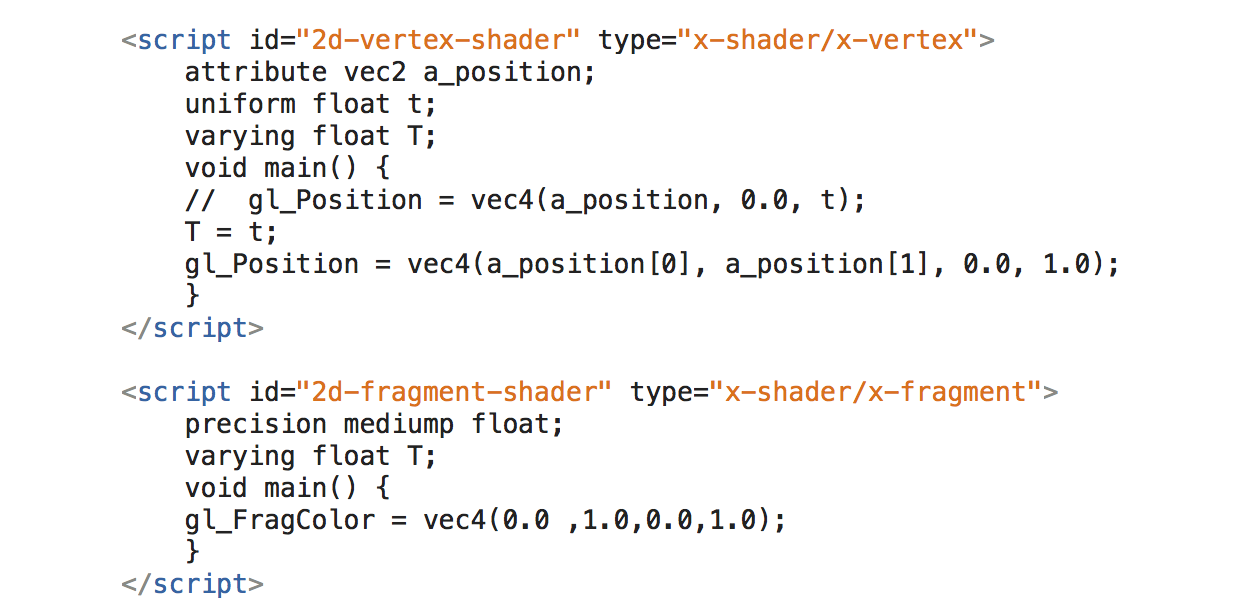
\includegraphics[scale=0.56]{images/shader}
\end{center}
\end{block}
\end{frame}

\begin{frame}
    \frametitle{Basis}
\framesubtitle{}
    \begin{block}{Basis}
Sind $b_1, b_2, b_3$ linear unabhängig, dann heisst die geordnete Menge
$ B = \{ b_1 , b_2, b_3\}$ Basis des $\mathbb{R}^3$.
\end{block}
 \begin{block}{Basisdarstellung}
Für $v \in \mathbb{R}^3$ heisst
\begin{eqnarray*}
& \theta_B : \mathbb{R}^3 \to  \mathbb{R}^3 \\
& \theta_B(v) =  \begin{pmatrix}
 \lambda_1 \\ \lambda_2 \\ \lambda_3
\end{pmatrix}  \\
& \text{mit } \lambda_1 \cdot b_1 + \lambda_2 \cdot b_2  + \lambda_3 \cdot b_3 = v 
\end{eqnarray*}
Darstellung von $v$ bezüglich der Basis $B$.
\end{block}

\end{frame}

\begin{frame}
    \frametitle{Basiswechsel}
\framesubtitle{}
\begin{block}{Basiswechsel berechnen}
\begin{eqnarray*}
& \theta_B(v) =  M_B \cdot v, \; \; M_B :=  \begin{pmatrix}
 b_1 & b_2 &  b_3
\end{pmatrix}^{-1} \text{(column major)}
\end{eqnarray*}
\end{block}

\begin{block}{Basiswechsel}
Seien $B:= \{ b_1, \hdots , b_n \}$ und $B':= \{ b'_1, \hdots , b'_n \}$ zwei Basen des $\mathbb{R}^n$.
Dann heißt $M_{B}^{B'} : = M_{B'}  \cdot M_{B}^{-1} $ die Basiswechselmatrix von $B$ nach $B'$. Wir haben also folgende Situation:
\begin{align*}
\xymatrix{
\mathbb{R}^n  \ar[d]^{I_n} &  & \ar[ll]^{M_B^{-1}} \mathbb{R}^n \ar[d]^{M_{B}^{B'}} \\
\mathbb{R}^n  \ar[rr]^{M_{B'}} & &  \mathbb{R}^n
}
\end{align*}
\end{block}
\end{frame}


\begin{frame}
    \frametitle{Skalarprodukt}
\framesubtitle{}
\begin{block}{Skalarproduktt}
$\langle v ,w \rangle := v^t \cdot w = \sum_{i=1}^{3} v_i \cdot w_i$ \\
Zwei vom Nullvektor verschiedene Vektoren $u,v \in \mathbb{R}^n$ heißen orthogonal, falls $<u,v> = 0$ ist. 
\end{block}
\begin{block}{Norm}
$||v || : = \sqrt{\langle v ,v \rangle} := v^t \cdot w = \sqrt{\sum_{i=1}^{3} v_i ^{2}}$ \\
Ein Vektor $v$ heißt normal, falls $||v|| = 1$ ist.
Ist $w$ ein beliebiger Vektor, so heißt $\frac{1}{||w||} w$ die Normalisierung von $w$, denn er ist normal.
\end{block}
\begin{block}{Satz}
Für den von zwei Vektoren $u,v$ eingeschlossenen Winkel $\varphi$ gilt:
\begin{align*}
\cos(\varphi) = \frac{<u,v>}{||u|| \cdot ||v||}
\end{align*}
\end{block}
\end{frame}


\begin{frame}
    \frametitle{Kreuzprodukt}
\framesubtitle{}
\begin{block}{Kreuzprodukt}
Für $u = \begin{pmatrix} u_1 \\ u_2 \\ u_3 \end{pmatrix}$ und $v= \begin{pmatrix} v_1 \\ v_2 \\ v_3 \end{pmatrix}$ heißt
\begin{align*}
u \times v :=  \begin{pmatrix} u_2 v_3 - u_3v_2  \\ u_3 v_1 - u_1v_3 \\ u_1 v_2 - u_2 v_1\end{pmatrix} 
\end{align*}
das Kreuzprodukt von $u$ und $v$.
Es gilt
\begin{itemize}
\item $<u \times v, u> =  <u \times v, v> = 0$ 
\item $u \times v = - (v \times u)$
\item $u \times v = 0$ genau dann, wenn $u$ und $v$ linear abhängig sind.
\end{itemize}
\end{block}
\end{frame}

\begin{frame}
    \frametitle{Orthonormalbasis}
\framesubtitle{}
\begin{block}{Orthonormalbasis}
Eine Basis  $B:= \{ b_1, b_2 , b_3 \}$ heißt Orthonormalbasis (kurz ONB), falls 
\begin{align*}
<b_i, b_j> = \begin{cases}  1 \; \text{falls }  i = j  \\ 0 \; \text{sonst}\end{cases}
\end{align*}
gilt. Insbesondere sind alle $b_i$ normal.
\end{block}
\end{frame}


\begin{frame}
    \frametitle{Orthonormalbasis}
\framesubtitle{}
\begin{block}{Basis-Wechsel-Matrix}
Ist  $B:= \{ b_1, \hdots , b_n \}$  eine ONB, so gilt
\begin{align*}
M_{B}^{-1} = M_{B}^t
\end{align*}
\end{block}
\begin{block}{Drehungen}
Eine Matrix $O \in \mathbb{M}^{n \times n}$ heißt orthogonal, falls
$O^{-1} = O^t$ ist.  Sie ist genau dann  orthogonal, falls
\begin{align*}
\det(O) \in  \{-1, 1 \} \; .
\end{align*}
Ist $\det(O) = 1$, so nennen wir $O$ eine Drehung und 
$SO(n) := \{ O \in \mathbb{M}^{n \times n} | \det(O) = 1\}$ die Drehgruppe (oder auch spezielle orthogonale Gruppe).
\end{block}

\end{frame}


\begin{frame}
    \frametitle{Orthonormalbasis}
\framesubtitle{}
\begin{block}{Basis-Wechsel-Matrix}
Sei $O \in \mathbb{M}^{n \times n}$ eine orthogonale Matrix, dann gilt für alles $v,w \in \mathbb{R}^n$
\begin{align*}
< O \cdot v \; , \;  O \cdot w > = <v \; , \; w>
\end{align*}
und somit insbesondere 
\begin{align*}
|| O \cdot v|| = ||v|| \; .
\end{align*}
\end{block}

\end{frame}


\begin{frame}
    \frametitle{Orthonormalbasis}
\framesubtitle{}
\begin{block}{Eulerwinkel}
Jede Drehung  $O \in SO(3)$  lässt sich zerlegen in ein Produkt
\begin{align*}
O = 
\begin{pmatrix}
1 & 0 & 0 \\
0 & \cos(\phi) & \pm \sin(\phi) \\ 
 0 & \mp \sin(\phi) & \cos(\phi)
\end{pmatrix}
\cdot
\begin{pmatrix}
 \cos(\psi) & 0 &   \sin(\psi) \\ 
0 & 1 & 0 \\ 
- \sin(\psi) & 0& \cos(\psi)
\end{pmatrix} \\
\cdot \begin{pmatrix}
 \cos(\xi) &  \sin(\xi)  & 0\\ 
 - \sin(\xi) & \cos(\xi) & 0 \\
0 & 0 & 1 
\end{pmatrix} 
\end{align*} 
Die Winkel $\phi, \psi, \xi$ heißen  Eulerwinkel. 
\end{block}

\end{frame}


\begin{frame}
    \frametitle{Orthonormalbasis}
\framesubtitle{}
\begin{figure}[H]
    \centering
    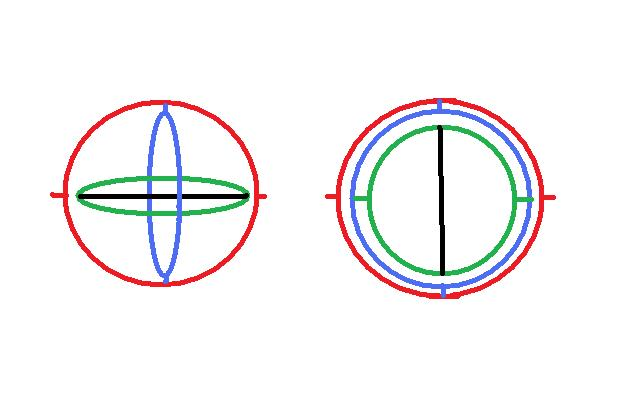
\includegraphics[width=0.6\textwidth]{images/gimbalLock.jpg}

\end{figure}
\begin{block}{Eulerwinkel}
Die  Zerlegung  $O \in SO(3)$  einer Drehung in obiges Produkt ist  nicht eindeutig.
Ein anschauliches Beispiel dafür liefert der sogenannte "Gimbal lock". $SO(3)$ ist also nicht das Produkt von drei Intervallen sondern
es ist $SO(3) = S^{3}/ \{ \pm 1 \}$.



\end{block}

\end{frame}


\begin{frame}
    \frametitle{Affiner Raum}
\framesubtitle{}
\begin{block}{Affiner Raum}
Der Affine Raum $\mathbb{A}^3$ ist ein Tupel $\bigl( \mathbb{R}^3, (\mathbb{R}^3, + , \cdot ) \bigr )$
zusammen mit den Abbildung 
\begin{align*}
\text{---} : \mathbb{R}^3 \times \mathbb{R}^3  & \to (\mathbb{R}^3, + , \cdot ) \\
\overline{PQ} & := Q-P  
\end{align*}
und
\begin{align*}
+ : \mathbb{R}^n \times (\mathbb{R}^3, + , \cdot )   & \to  \mathbb{R}^3\\
\begin{pmatrix}
P_1 \\ \vdots \\ P_3
\end{pmatrix} + \begin{pmatrix}
v_1 \\ \vdots \\ v_3
\end{pmatrix} & := \begin{pmatrix}
P_1  + v_1 \\ \vdots \\ P_3 + v_3
\end{pmatrix}   \;.
\end{align*}

\end{block}

\end{frame}


\begin{frame}
    \frametitle{Affiner Raum}
\framesubtitle{}
\begin{block}{Affiner Raum}
Die Elemente (Vektoren) aus $\mathbb{R}^3$ nennt man auch  Punkte in Abgrenzung zu den Vektoren aus $(\mathbb{R}^3, + , \cdot )$.  
Für Punkte $P,Q \in \mathbb{R}^3$ ist also $\overline{PQ}$ ein Vektor, auch Verbindungsvektor genannt.
\end{block}

\end{frame}


\begin{frame}
    \frametitle{Affiner Raum}
\framesubtitle{}
\begin{block}{Affine basis}
Ist $B:= \{b_1, b_2 , b_3 \}$ eine Basis des Vektorraums  $(\mathbb{R}^3, + , \cdot )$ und $P \in \mathbb{A}$ ein Punkt, so nennen wir das Tupel
$(P, B)$ eine affine Basis. Für jeden Punkt $Q$ gibt es dann also Skalare $\lambda_1,\hdots ,\lambda_n$ mit 
\begin{align*}
Q = P + \sum_{i=1}^{3} \lambda_i \cdot b_i  \; .
\end{align*}
Der Punkt $\theta_{(P,B)}(Q):= \begin{pmatrix}  \lambda_1 \\   \lambda_2 \\  \lambda_3 \end{pmatrix}$ heißt die Darstellung von $Q$ bezüglich der affinen Basis $(P,B)$. 
\end{block}

\end{frame}



\begin{frame}
    \frametitle{Affiner Raum}
\framesubtitle{}
\begin{block}{Affine Abbildung}
Abbildungen der Form
\begin{align*}
\phi &: \mathbb{A}^3 \to \mathbb{A}^3 \\
\phi(P) & := A \cdot P + t
\end{align*} 
mit $A \in M^{3 \times 3}$ und $t \in (\mathbb{R}^3, + , \cdot )$ heißen affine Abbildungen.
Insbesondere heißt eine affine Abbildung mit $A = I_3$ und $t \neq 0$ Translation.
\end{block}
\begin{block}{Abstand}
Der Abstand von  $P,Q \in \mathbb{A}$  ist definiert durch
\begin{align*}
d : \mathbb{A}^3 \times \mathbb{A}^3 \to \mathbb{R} \\
d(P,Q) := || \overline{PQ} || \; .
\end{align*}
\end{block}

\end{frame}



\begin{frame}
    \frametitle{Affiner Raum}
\framesubtitle{}
\begin{block}{Affiner Basiswechsel}

Sind $(P,B:= \{b_1, \hdots , b_n \})$  und $(P',B':= \{b'_1, \hdots , b'_n \})$ zwei affine Basen  und definieren wir 
die Abbildung
\begin{align*}
\theta_{(P,B)} & :  \mathbb{A}^n \to \mathbb{A}^n \\
\theta_{(P,B)}(Q) & := M_B \cdot Q - M_B \cdot P  =  M_B (Q -  P ),
\end{align*}
so erhalten wir analog zu der Situation in Vektorräumen
\begin{align*}
\xymatrix{
\mathbb{A}^n  \ar[d]^{\text{id}} &  & \ar[ll]^{\theta_{(P,B)}^{-1}} \mathbb{A}^n \ar[d]^{\theta_{(P,B)}^{(P',B')}} \\
\mathbb{A}^n  \ar[rr]^{\theta_{(P',B')}} & &  \mathbb{A}^n
}
\end{align*}
mit $\theta_{(P,B)}^{(P',B')} (Q) :=   \theta_{(P',B')} \biggl ( \theta_{(P,B)}^{-1} (Q) \biggr)$.
\end{block}

\end{frame}



\begin{frame}
    \frametitle{Homogene Koordinaten}
\framesubtitle{}
\begin{block}{Projektier Raum}

Der projektive  Raum ist definiert als
\begin{align*}
\mathbb{P}^3 := \mathbb{R}^{4} - \{ 0\} / \sim \\
v \sim w \Leftrightarrow v = \lambda w \text{ für ein } \lambda \neq 0 \in \mathbb{R} \; . 
\end{align*}
\end{block}
\end{frame}

\begin{frame}
    \frametitle{Homogene Koordinaten}
\framesubtitle{}
\begin{block}{Homogene Koordinaten}
Wir haben die Abbildung
\begin{align*}
\mathbb{A}^3 & \to \mathbb{P}^3 \\
\begin{pmatrix} p_1 \\ p_2 \\ p_3 \end{pmatrix} & \mapsto \begin{pmatrix} p_1 \\ p_2 \\ p_3  \\  1\end{pmatrix} 
\end{align*}
und nennen das Bild eines Punktes unter dieser Abbildung die homogenen Koordinaten.
\end{block}
\end{frame}

\begin{frame}
    \frametitle{Homogene Koordinaten}
\framesubtitle{}
\begin{block}{Homogene Koordinaten}
Auf der Menge der homogenen Koordinaten haben wir die Umkehrabbildung
\begin{align*}
& \mathbb{P}^3 - \Biggl \{\begin{pmatrix} p_1 \\ p_2 \\ p_3  \\ p_4 \end{pmatrix}\Bigg | \; p_{4} = 0 \Biggr \}   \to \mathbb{A}^3 \\
& \begin{pmatrix} p_1 \\ p_2 \\ p_3  \\  p_{4} \end{pmatrix}   \mapsto \begin{pmatrix}  \frac{p_1}{ p_{4}} \\ \frac{p_2}{ p_{4}}  \\ \frac{p_3}{ p_{4}}  \end{pmatrix}  \; .
\end{align*}
\end{block}
\end{frame}


\begin{frame}
    \frametitle{Homogene Koordinaten}
\framesubtitle{}
\begin{block}{Ferne Punkte}
Die Menge der Punkte $F_3 := \Biggl \{\begin{pmatrix} p_1 \\ p_2 \\ p_3  \\ p_4 \end{pmatrix}\Bigg | \; p_{4} = 0 \Biggr \} $ heissen unendlich ferne Punkte.

\begin{align*}
 \begin{pmatrix} p_1 \\ p_2 \\ p_3  \\ 0 \end{pmatrix}  =\lim_{n \to \infty} \begin{pmatrix} p_1 \\ p_2 \\ p_3  \\ \frac{1}{n} \end{pmatrix}  \cong  \lim_{n \to \infty} n \cdot  \begin{pmatrix} p_1 \\ p_2 \\ p_3 \end{pmatrix} 
\end{align*}
\end{block}

\begin{block}{Identifikation der fernen Punkte}
Es ist $F_3 \cong \mathbb{P}^2$
\end{block}
\end{frame}


\begin{frame}
    \frametitle{Homogene Koordinaten}
\framesubtitle{}
\begin{block}{Zerlegung des projektiven Raumes}
Der projektive Raum ist damit die Vereinigung des Affinen Raumes und den unendlich fernen Punkten. "Parallelen schneiden sich in den unendlich fernen Punkten".
Es gilt also 
\begin{align*}
& \mathbb{P}^3 = \mathbb{A}^3 \cup F_3 = \mathbb{A}^3  \cup \mathbb{P}^2 =  \mathbb{A}^3  \cup \mathbb{A}^2 \cup F_2  \\  
& =\mathbb{A}^3  \cup \mathbb{A}^2 \cup  \mathbb{P}^1 =   \mathbb{A}^3  \cup \mathbb{A}^2 \cup  \mathbb{S}^1/ \{ \pm  1\} \\
& =  \mathbb{A}^3  \cup \mathbb{A}^2 \cup  \mathbb{S}^1
\end{align*}
\end{block}
\end{frame}




\begin{frame}
    \frametitle{Homogene Koordinaten}
\framesubtitle{}

\begin{center}
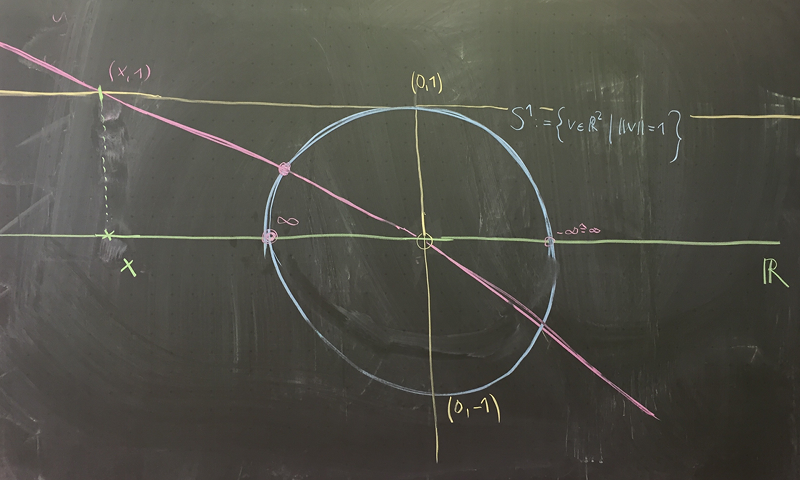
\includegraphics[scale=0.40]{images/proj2.png}
\end{center}
\end{frame}

\begin{frame}
    \frametitle{Homogene Koordinaten}
\framesubtitle{}
\begin{block}{Projektive Abbildungen}
Wir können damit und mit der Definition der Matrix-Vektor-Multiplikation eine affine Abbildung 
\begin{align*}
\phi : \mathbb{A}^{3} \to \mathbb{A}^{3} \\
\phi(v):=  A \cdot v + t
\end{align*}
in homogenen Koordinate ausdrücken durch eine Matrizenmultiplikation
\begin{align*}
\begin{pmatrix} v \\ 1\end{pmatrix} \mapsto \begin{pmatrix}  A  & t  \\ 0 &1\end{pmatrix} \cdot  \begin{pmatrix} v \\ 1\end{pmatrix}  =    \begin{pmatrix}  A v +t   \\ 1\end{pmatrix}  \; .
\end{align*}
\end{block}
\end{frame}

\begin{frame}
    \frametitle{Homogene Koordinaten}
\framesubtitle{}
\begin{center}
    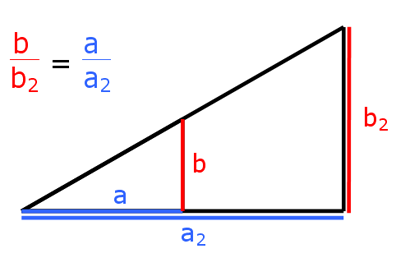
\includegraphics[width=0.35\textwidth]{images/strahlensatz}
\end{center}
\begin{block}{Zentralprojektion}
Die Matrizen
\begin{align*}
K_{persp_{xy}} := \begin{pmatrix}  
1   &  0 & 0 & 0  \\
0   &  1 & 0 & 0  \\
0   &  0 & 1 & 0  \\
0   &  0 & \frac{1}{d} & 0 
\end{pmatrix} ,
K_{orth_{xy}} := \begin{pmatrix}  
1   &  0 & 0 & 0  \\
0   &  1 & 0 & 0  \\
0   &  0 & 0 & 1  
\end{pmatrix} \; ,
\end{align*}
realisieren die Zentralprojektion auf die Ebene parallel zur $X-Y$-Ebene und Augenpunkt im Ursprung mit Augendistanz $d$ in homogenen Koordinaten.


\end{block}
\end{frame}

\begin{frame}
    \frametitle{Homogene Koordinaten}
\framesubtitle{}
\begin{block}{Zentralprojektion}
Die Zentralprojektion auf die Ebene parallel zur $X-Y$-Ebene und Augenpunkt im Ursprung mit Augendistanz $d$ durch die Hintereinanderausführung folgender Abbildungen darstellen:
\begin{align*}
& persp_{xy} :\mathbb{A}^3   \to \mathbb{P}^3    \to  \mathbb{P}^3    \to \mathbb{P}^2    \to \mathbb{A}^2  \\
&\begin{pmatrix} x \\ y \\ z \end{pmatrix} \mapsto \begin{pmatrix} x \\ y \\ z \\ 1 \end{pmatrix}   \mapsto K_{persp_{xy}} \cdot  \begin{pmatrix} x \\ y \\ z \\ 1 \end{pmatrix} =   \begin{pmatrix} x \\ y \\ z \\ \frac{z}{d}  \end{pmatrix} \\
 & \mapsto K_{orth_{xy}} \cdot   \begin{pmatrix} x \\ y \\ z \\ \frac{z}{d}  \end{pmatrix}=   \begin{pmatrix} x \\ y \\ \frac{z}{d} \end{pmatrix}   \mapsto 
 \begin{pmatrix}  \frac{x}{\frac{z}{d} } \\   \frac{y}{\frac{z}{d} } \end{pmatrix}
 \end{align*}

\end{block}
\end{frame}


\begin{frame}
    \frametitle{Homogene Koordinaten}
\framesubtitle{}
\begin{block}{Clipping Koordinaten}

\begin{align*}
P := \begin{pmatrix}  
\frac{n}{r}  &  0 & 0  & 0  \\
0   &  \frac{n}{t} & 0 & 0  \\
0   &  0 & \frac{-f-n}{f-n} & \frac{-2\cdot f \cdot n}{f-n}  \\
0   &  0 & -1 & 0  
\end{pmatrix}  \; .
\end{align*} 


$MVP := Model View Projection Matrix$

\end{block}
\begin{center}
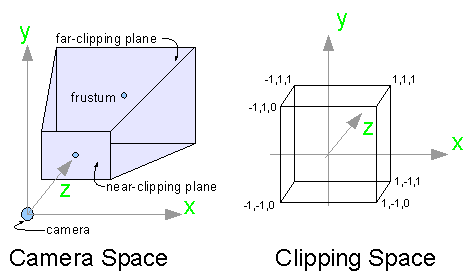
\includegraphics[scale=0.40]{images/projection}
\end{center}
\end{frame}





\begin{frame}
    \frametitle{Rasterung}
\framesubtitle{}
\begin{block}{Bresenham}

\begin{itemize}
\item{Der Algorithmus wurde 1962 von Jack Bresenham, damals Programmierer bei IBM, entwickelt. }

\item{Rundungsfehler, die durch die Diskretisierung von kontinuierlichen Koordinaten entstehen, werden minimiert. }
\item{Einfach implementierbar.}

\item{Kommt mit der Addition von ganzen Zahlen als komplexeste Operation, und somit ohne Multiplikation, Division und Gleitkommazahlen. }

\item{Durch eine geringfügige Erweiterung lässt sich der ursprüngliche Algorithmus, der für Geraden entworfen wurde, auch für die Rasterung von Kreisen verwenden. Sogar die Quadratterme, die beim Kreis vorkommen, lassen sich rekursiv ohne jede Multiplikation aus dem jeweils vorhergehenden Term ableiten.}
\end{itemize}
\end{block}
\end{frame}


\begin{frame}
    \frametitle{Rasterung}
\framesubtitle{}
\begin{block}{Bresenham}

  Die Strecke $S = \overline{PQ} \in \mathbb{R}^n$ soll auf ein 
    ($n$-dimensionales Pixel-) Raster abgebildet werden

    \begin{equation*}\begin{matrix}
        P = \begin{pmatrix} x_0 \\ y_0 \end{pmatrix} & 
        Q = \begin{pmatrix} x_1 \\ y_1 \end{pmatrix} & 
        \forall x_i, y_i \in \mathbb{R}
    \end{matrix}\end{equation*}
    \begin{equation*}
        M_p = \left( x_p + 1,~ y_p + \frac{1}{2} \right)
    \end{equation*}


\end{block}
\begin{center}
    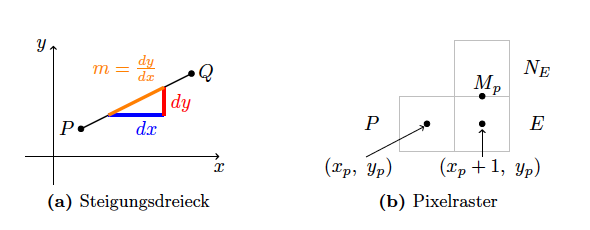
\includegraphics[width=0.8\textwidth]{images/bresenham}
\end{center}
\end{frame}


\begin{frame}
    \frametitle{Rasterung}
\framesubtitle{}

\begin{block}{Bresenham}

    \begin{equation*}
        M_p ~\Big\{~ \begin{matrix}
            \textrm{oberhalb}~ \overline{PQ} &\Rightarrow& \textrm{wähle}~ E \\ 
            \textrm{unterhalb}~ \overline{PQ} &\Rightarrow& \textrm{wähle}~ N_E 
        \end{matrix}
    \end{equation*}\\
  
    \begin{equation*}\begin{matrix}
        F\left(x,~ y\right) & := & dy \cdot x - dx \cdot y + dx \cdot b 
    \end{matrix}\end{equation*}

\begin{equation*}
\begin{matrix}
        (x,~ y) \in y = mx + b & \Leftrightarrow & F\left(x,~ y\right) = 0 \\
        & \textrm{bzw.} & \\
        F\left(x,~ y\right) & \Bigg\{ & \begin{matrix}
            = 0 & \left(x,~ y\right) \textrm{liegt auf}~ S \\
            > 0 & \left(x,~ y\right) \textrm{liegt unterhalb von}~ S \\
            < 0 & \left(x,~ y\right) \textrm{liegt oberhalb von}~ S \\
        \end{matrix}
    \end{matrix}\end{equation*}
   \end{block}
\end{frame}


\begin{frame}
    \frametitle{Rasterung}
\framesubtitle{}
\begin{block}{Bresenham}
\begin{equation*}\begin{matrix}
        D_p & := & 2 \cdot F\left(M_p\right) \\
         \end{matrix}\end{equation*}
    1. Fall: $D_p < 0 ~\Rightarrow~$ Nachfolgepixel ist $E$
    \begin{equation*}\begin{matrix}
        D_E & = & 2 \cdot F\left(M_E\right) \\
        & = & 2 \cdot F\left(x_p + 2,~ y_p + \frac{1}{2}\right) \\
        & = & dy \cdot \left(2 x_p + 4\right) 
            - dx \cdot \left(2 y_p + 1\right) 
            + 2 \cdot b \cdot dx \\
        & = & D_p + \bigtriangleup_E \\
        & \textrm{mit} & \bigtriangleup_E := 2 \cdot dy
    \end{matrix}\end{equation*}
    2. Fall: $D_p \ge 0 ~\Rightarrow~$ Nachfolgepixel ist $NE$ \\
    \begin{equation*}\begin{matrix}
        D_{NE} & = & 2 \cdot F\left( M_{NE} \right) \\
        & = & D_p + \bigtriangleup_{NE} \\
        & \textrm{mit} & \bigtriangleup_{NE} := 2dy - 2dx
    \end{matrix}\end{equation*}
\end{block}
\end{frame}



\begin{frame}
    \frametitle{Rasterung}
\framesubtitle{}
\begin{center}
    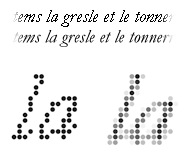
\includegraphics[width=0.5\textwidth]{images/Antialiasing}
\end{center}
\begin{block}{Anti Aliasing}
Kantenglättung z.B. mit Gaußfilter.
\end{block}
\end{frame}



\begin{frame}
    \frametitle{Rasterung}
\framesubtitle{}
\begin{center}
    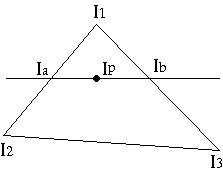
\includegraphics[width=0.4\textwidth]{images/gouraud_scanline.png}
\end{center}
\begin{block}{Interpolation}
GLSL interpoliert Werte innerhalb eines Fragmentes linear zwischen den im Vertex-Shader gesetzten Werten.
Dies kann  zum Beispiel mit Hilfe eines Sweepline-Algorithmus realisiert werden.


\end{block}
\end{frame}



\begin{frame}
    \frametitle{Photometrie}
\framesubtitle{}
\begin{block}{Fläche}

Ein Fläche (Parametrisierung) ist  eine  Abbildung
\begin{align*}
s: U \subset \mathbb{R}^2 \to \mathbb{R}^3 \\
s(u,v) := \begin{pmatrix} x(u,v) \\ y(u,v) \\ z(u,v) \end{pmatrix} 
\end{align*} 
bei der die Abbildungen $x, y, z : U \subset \mathbb{R}^2 \to \mathbb{R}$ stetig sind. Sie heißt differenzierbar, falls die partiellen Ableitungen
\begin{align*}
\frac{\partial}{\partial u} s(u,v) = \begin{pmatrix}  \frac{\partial}{\partial u} x(u,v) \\  \frac{\partial}{\partial u} y(u,v) \\  \frac{\partial}{\partial u} z(u,v) \end{pmatrix}, \;
\frac{\partial}{\partial v} s(u,v) =  \begin{pmatrix} \frac{\partial}{\partial v} x(u,v) \\ \frac{\partial}{\partial v} y(u,v) \\ \frac{\partial}{\partial v} z(u,v) \end{pmatrix}
\end{align*}
existieren. 
\end{block}
\end{frame}


\begin{frame}
    \frametitle{Photometrie}
\framesubtitle{}
\begin{block}{Tangentialraum}

Die Ebene 
\begin{align*}
T_s(u,v) :=  \{ s(u,v) + \lambda \cdot \frac{\partial}{\partial u} s(u,v) + \mu \cdot \frac{\partial}{\partial v} \; | \; \lambda, \mu \in \mathbb{R} \}
\end{align*}
heißt Tangentialebene am Punkt $(u,v)$ und  der Vektor 
\begin{align*}
n (u,v):= \frac{\partial}{\partial u} s(u,v) \times \frac{\partial}{\partial v} s(u,v) \; ,
\end{align*}
welcher Senkrecht auf dieser Ebene steht,  die Normale.
\end{block}
\end{frame}

\begin{frame}
    \frametitle{Photometrie}
\framesubtitle{}
\begin{block}{Oberflächenintegral}

Das OberflächenIntegral ist definiert durch
\begin{align*}
\int_S d \omega:= \int_U ||n(u,v)|| \; dU \;.
\end{align*} 
und  analog
\begin{align*}
\int_S f \;  d \omega:= \int_U f(s(u,v)) \cdot ||n(u,v)|| \; dU \;.
\end{align*} 
für eine Funktion $f: S \to \mathbb{R}$.
Man nennt $d \omega$ beziehungsweise $ ||n(u,v)||$ das infinitessimale Flächenelement.
\end{block}
\end{frame}

\begin{frame}
    \frametitle{Photometrie}
\framesubtitle{}
\begin{block}{Fubini}
Ist $U = U_1 \times U_2 \in \mathbb{R}^2$ und $f: U \to \mathbb{R}$ eine integrierbare Funktion, so gilt
\begin{align*}
\int_U f \; d(U_1 \times U_2) = \int_{U_1} \int_{U_2} f  \;  dU_2 dU_1   = \int_{U_1} \int_{U_2} f  \;  dU_1 dU_2 \;.
\end{align*} 
\end{block}
\end{frame}


\begin{frame}
    \frametitle{Photometrie}
\framesubtitle{}
\begin{block}{Die  Sphäre $S^2$}
\begin{align*}
& s:  [0, \pi) \times  [0, 2 \pi)  \to \mathbb{R}^3 , \;
  s(u,v) :=  
 \begin{pmatrix}  \sin(u) \cos(v) \\   \sin(u) \sin(v) \\   \cos(u)  \end{pmatrix} \\
& \frac{\partial}{\partial u} s(u,v) =  \begin{pmatrix}  \cos(u) \cos(v) \\   \cos(u) \sin(v) \\   -\sin(u)  \end{pmatrix} , 
\frac{\partial}{\partial v} s(u,v) =  \begin{pmatrix}  -\sin(u) \sin(v) \\   \sin(u) \cos(v) \\   0  \end{pmatrix} \\
& ||\frac{\partial}{\partial u} s(u,v) \times \frac{\partial}{\partial v} s(u,v) || = sin(u)
\end{align*} 
\begin{align*}
& \int_{S^2} d\omega  = \int_{[0, \pi) \times  [0, 2 \pi) } sin(u) d(u \times v) =   \int_{[0, 2 \pi) }   \int_{[0, \pi) } sin(u) du dv \\ 
& = 4 \pi
\end{align*} 

\end{block}
\end{frame}


\begin{frame}
    \frametitle{Photometrie}
\framesubtitle{}
\begin{center}
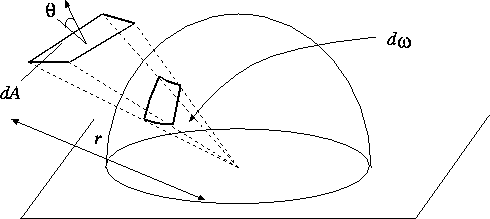
\includegraphics[scale=0.30]{images/solidangle}
\end{center}

\begin{block}{Transformationsformel}


\begin{align}
& d\omega =  \frac{1}{r^2} \cdot  \cos(\theta) dA, \;  \pi(x):=  \frac{x}{||x||}  \\
& V(x,y) := \begin{cases}
1 \text{ falls } \overline{xy} \cap (A -\{x,y\}) = \emptyset \\
0 \text{ sonst }
\end{cases} \\
& \int_{\pi(A)} f \cdot   d\omega  =  \int_{A} f  \cdot \frac{1}{r^2} \cdot  \cos(\theta) \cdot V(a, 0)  \; dA \; ,
\end{align}


\end{block}
\end{frame}


\begin{frame}
    \frametitle{Photometrie}
\framesubtitle{}
\begin{center}

    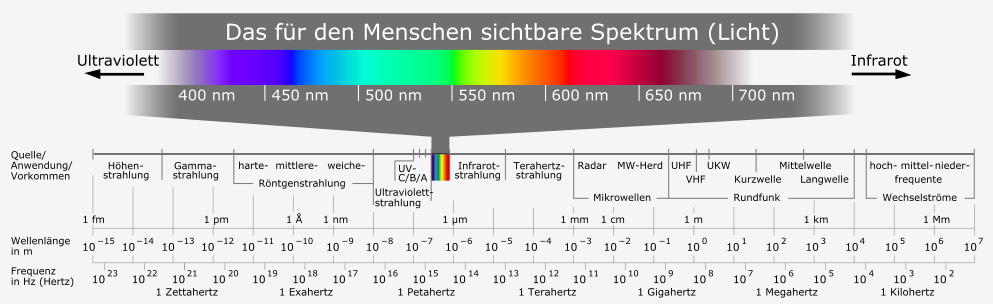
\includegraphics[width=1.0\textwidth]{images/Electromagnetic_spectrum_c.png}
\end{center}
\begin{block}{Lichtenergie}

Die Lichtenergie wird durch einen Strom von Photonen erzeugt. Die Energie eines Photons ist 
durch $E=h \cdot f$, mit  $h$ das konstante Planksche Wirkungsquantum und $f$ die Frequenz der Welle (Welle-Teilchen Dualismus).  


\end{block}
\end{frame}


\begin{frame}
    \frametitle{Photometrie}
\framesubtitle{}
\begin{block}{Strahlungsleistung}

Die Strahlungsleistung $\phi = \frac{d Q}{dt}$ ist die von einem Photonenstrom übertragenen Energie $Q$ pro Zeit. 
Für monochromes Licht mit der Frequenz $f$ und Teilchenstrom $ \frac{d N}{dt} $ ergibt sich $\phi = h \cdot  \frac{d N}{dt}  \cdot f$.



\end{block}
\end{frame}


\begin{frame}
    \frametitle{Photometrie}
\framesubtitle{}
\begin{center}
    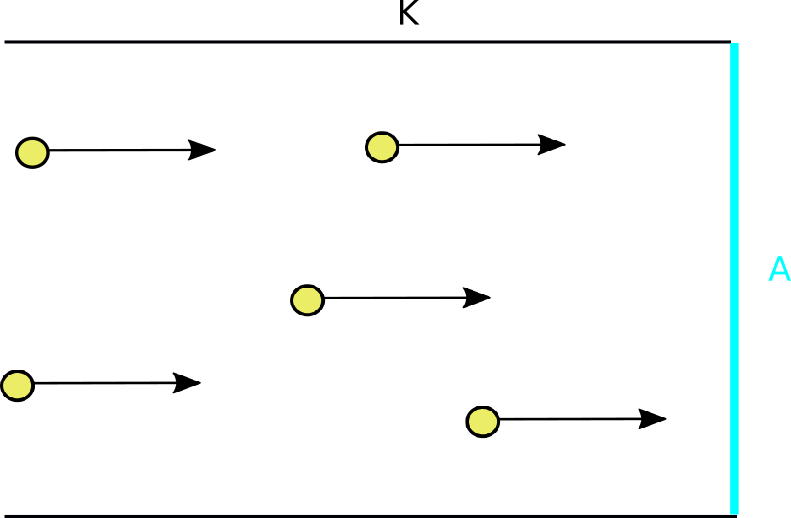
\includegraphics[width=0.4\textwidth]{images/Partikelstrom.png}
\end{center}
\begin{block}{ Strahldichte}

Durch einen Kanal $K$ bewegen  sich Teilchen mit gleichförmiger Geschwindigkeit $L$ (Lichtgeschwindigkeit)  und  Dichte $\eta$.
Die Anzahl der Teilchen $N$, die die Fläche $A$ bezüglich eines Zeitintervalles $[0,t]$ passieren, ist gegeben durch
\begin{align}
& N_A([0,t]) := \eta * ||L||  *   \text{Flächeninhalt}(A) *   t 
\end{align}
\end{block}
\end{frame}

\begin{frame}
    \frametitle{Photometrie}
\framesubtitle{}

\begin{center}

    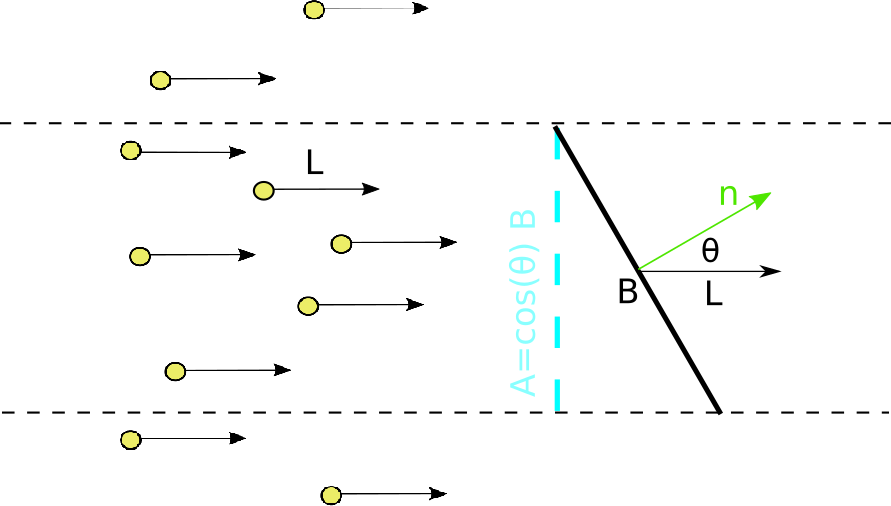
\includegraphics[width=0.5\textwidth]{images/Strahldichte.png}
\end{center}


\begin{block}{Strahldichte}
 Betrachtet man die allgemeinere Situation eines Flächenstückes $B$  in einem Teilchenstorm $N$, so ist die Anzahl gegeben durch 
\begin{align}
N_B([0,t]) := \eta * ||L||  * \cos(\alpha) *  \text{Flächeninhalt} (B) * t
 \end{align}


\end{block}
\end{frame}




\begin{frame}
    \frametitle{Photometrie}
\framesubtitle{}

\begin{block}{Strahldichte}
Bezeichnen wir mit 
\begin{align*}
L(B) = \frac{d}{dt \cdot \cos(\theta)}N_B([0,t]) = \eta * ||L||  *  \text{Flächeninhalt} (B) \; , 
 \end{align*}

so erhalten wir die   Strahldichte als Grenzwert
\begin{align*}
L(x, n):= \lim_{B -> x} L(B)
 \end{align*}
bei dem die Fläche $B$  zu einem Punkt $x$ zusammengezogen wird.  Die Strahlungsleistung aus einer Richtung $\theta$  am Punkt $x$ berechnet sich demnach durch $I(x, \theta) = L(x, \theta) \cdot \cos(\theta)$, was auch als Lambertsches Cosinusgesetz bezeichnet wird.
\end{block}
\end{frame}



\begin{frame}
    \frametitle{Photometrie}
\framesubtitle{}
  \begin{center}

    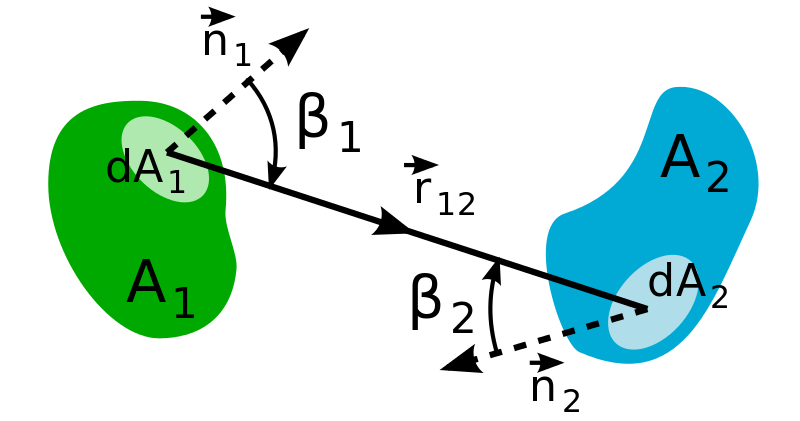
\includegraphics[width=0.45\textwidth]{images/Fotometrisches_Grundgesetz_Schema.png}
\end{center}


\begin{block}{Photometrisches Grundgesetz}


Die Strahlungsleistung $\phi:= \frac{ \partial Q}{\partial t}$, die von einer abstrahlenden Fläche $A_2$  auf eine Fläche $A_1$ übertragen wird, berechnet sich durch
\begin{align}
\phi = \int_{A_1} \int_{\pi_s(A_2)} L(x, \omega)\cdot \cos(\beta_1) d\omega  dA_1   \; ,
\end{align}
wobei $\theta$ der Winkel zwischen der Flächennormale am Punkt $x$ und der Richtung $\omega$ ist und $\pi_s(A_2)$ das sphärische Bild von $A_2$ ist.
\end{block}
\end{frame}


\begin{frame}
    \frametitle{Photometrie}
\framesubtitle{}
\begin{block}{Reflektionsgesetz}

\begin{align*}
\underbrace{L_r(x, \omega_r)}_{\substack{\text{Reflektierte Strahlung} \\ \text{in Richtungen $\omega_r$}}} =\underbrace{\int_{H^2} \underbrace{f_r (x, \omega, \omega_r)}_{\substack{\text{Reflektionseigenschaft} \\ \text{des Materials}}} \cdot  \underbrace{L_i(x, \omega) \cdot  \cos(\theta) }_{\substack{\text{Eingehende Strahlung} \\ \text{aus Richtung $\omega$}}} d\omega}_{\substack{\text{Summation über  alle } \\ \text{eingehenden Richtungen $\omega$}}} 
\end{align*}
  \begin{center}
    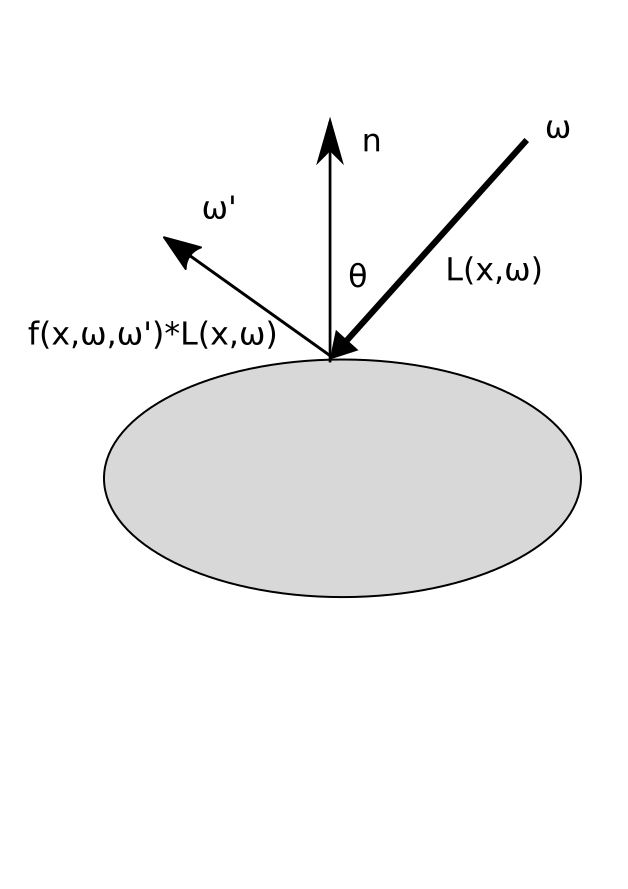
\includegraphics[width=0.3\textwidth]{images/brdf.png}
\end{center}
\end{block}
\end{frame}


\begin{frame}
    \frametitle{Raytracing}
\framesubtitle{}
\begin{block}{Rendergleichung}

\begin{align}
L_o(x, \omega_o) = L_e(x, \omega_o)  + \displaystyle \int_{H^2}f_r (x, \omega, \omega_0) \cdot L_i(x, \omega)  \cdot  \cos(\theta) d\omega \; ,
\end{align}
Ausgehend (\textbf{o}ut) = Emission (\textbf{e}mission) + Reflektion
\end{block}
\end{frame}



\begin{frame}
    \frametitle{Raytracing}
\framesubtitle{}

  \begin{center}
    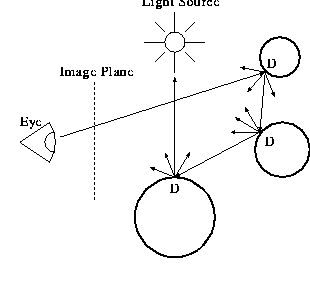
\includegraphics[width=0.7\textwidth]{images/rayTracing}
\end{center}

\end{frame}



\begin{frame}
    \frametitle{Raytracing}
\framesubtitle{}
\begin{block}{Rendergleichung 2-te Form}
 $\Omega$  Menge aller Flächen  in der Szene.
\begin{align*}
& V(x,y) := \begin{cases}
 1 \text{ falls } \overline{xy} \cap (\Omega -\{x,y\}) = \emptyset \\
0 \text{ sonst }
\end{cases} \\
& L_i(x, \omega_y) = V(x,y) \cdot L_o(y, \omega_x) \text{ (Energieerhaltung)} \\
& d\omega =  \frac{1}{||x -y||^2} \cdot  \cos(\theta_y) dA_y \\
& G(x,y) := V(x,y)  \frac{ \cos(\theta_x) \cdot  \cos(\theta_y)}{||x -y||^2} \\
& L_o(x, \omega_o) = L_e(x, \omega_o)  + \displaystyle \int_{\Omega} f_r (x, \overline{xy}, \omega_o) \cdot   L_o(y, \overline{xy})  \cdot  G(x,y) \cdot   dA_y \; .
\end{align*} 
\end{block}
\end{frame}


\begin{frame}
    \frametitle{Raytracing}
\framesubtitle{}
\begin{block}{Pfadformulierung}
\begin{align*}
&(T \circ  L)(x, \omega) :=  \displaystyle \int_{H^2}f_r (x, \omega, \omega_0) \cdot L(x, \omega)  \cdot  \cos(\theta) d\omega \; , \\
&L_e = (id - T) \circ L \; . \\
&L = (id - T)^{-1} \circ L_e  \\
&(id - T)^{-1}= \sum_{i= 0}^{\infty} T^i  \; .
\end{align*}

\end{block}
\end{frame}

\begin{frame}
    \frametitle{Monte Carlo Integration}
\framesubtitle{}
\begin{block}{Wahrscheinlichkeitsraum}
\begin{itemize}
\item  Menge $\Omega \subset \mathbb{R}^n$ deren Teilmengen Ereignisse genannt werden.
\item Funktion $\rho : \Omega \to \mathbb{R}$ mit $\int_{\Omega} \rho(\omega) d\omega = 1$ welche auch Wahrscheinlichkeitsdichte genannt wird.
\item Eine Abbildung $X: \Omega \to \mathbb{R}$ wird Zufallsvariable genannt.
\end{itemize}

Ist $X: \Omega \to \mathbb{R}$ eine  Zufallsvariable, dann heißt
\begin{align}
\mathbb{E}[X] := \int_{\Omega} X(\omega) \cdot \rho(\omega) d\omega 
\end{align}
Erwartungswert.
\end{block}
\end{frame}

\begin{frame}
    \frametitle{Monte Carlo Integration}
\framesubtitle{}
\begin{block}{Gesetz der großen Zahlen}
Ist $X: \Omega \to \mathbb{R}$ eine  Zufallsvariable mit Wahrscheinlichkeitsdichte $\rho: \Omega \to [0,1]$ und $\{ \omega_1, \cdots, \omega_N \}$ eine Stichprobe für $\rho$, so gilt:
\begin{align}
\frac{1}{N} \sum_{i= 0}^{N} X(\omega_i) \xrightarrow{ N \to \infty } \mathbb{E}[X] \text{ (in Wahrscheinlichkeit)}
\end{align}
\end{block}
\end{frame}

\begin{frame}
    \frametitle{Monte Carlo Integration}
\framesubtitle{}
\begin{block}{Stochastische Integration}

Ist $f: S \subset \Omega \to \mathbb{R}$ eine Funktion, so gilt für eine beliebige Wahrscheinlichkeitsdichte  $\rho: \Omega \to [0,1]$ und eine Stichprobe 
 $\{ \omega_1, \cdots, \omega_N \}$
\begin{align}
\frac{1}{N} \sum_{i= 0}^{N}  \frac{f(\omega_i)}{\rho(\omega_i)} \xrightarrow{ N \to \infty } \int_{\Omega} f(\omega) d\omega \text{ (in Wahrscheinlichkeit)} \; .
\end{align}
\end{block}

\begin{block}{Stochastische Integration}
Das Problem der Integration reduziert sich im Wesentlichen darauf viele Stichproben $\omega$ aus einer komplizierten  Verteilung  $\rho$ zu ziehen.
\end{block}

\end{frame}

\begin{frame}
    \frametitle{Rejectionsampling}
\framesubtitle{}

  \begin{center}
    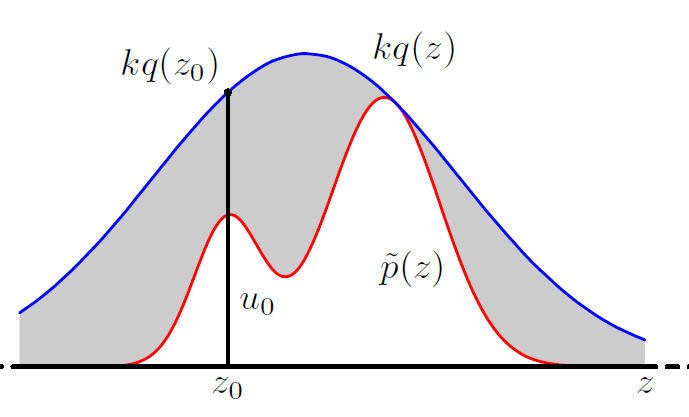
\includegraphics[width=0.9\textwidth]{images/rjsampling2}
\end{center}

\end{frame}



\begin{frame}
    \frametitle{Raytracing}
\framesubtitle{}
\begin{block}{Pathtracing}
Die Anwendung der Monte Carlo Integration auf die Pfadformulierung der Rendergleichung wird Pathtracing genannt.
\end{block}
\end{frame}




\begin{frame}
    \frametitle{Raytracing}
\framesubtitle{}
Wenige und viele samples im Vergleich

    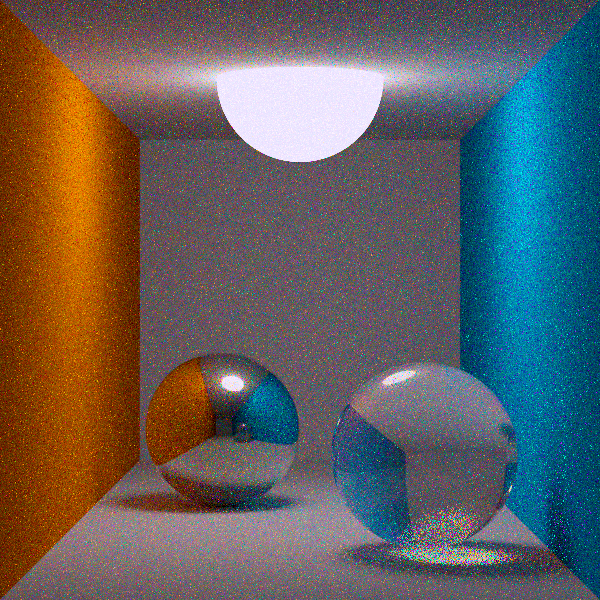
\includegraphics[width=0.45\textwidth]{images/Path_Tracing_Low}
    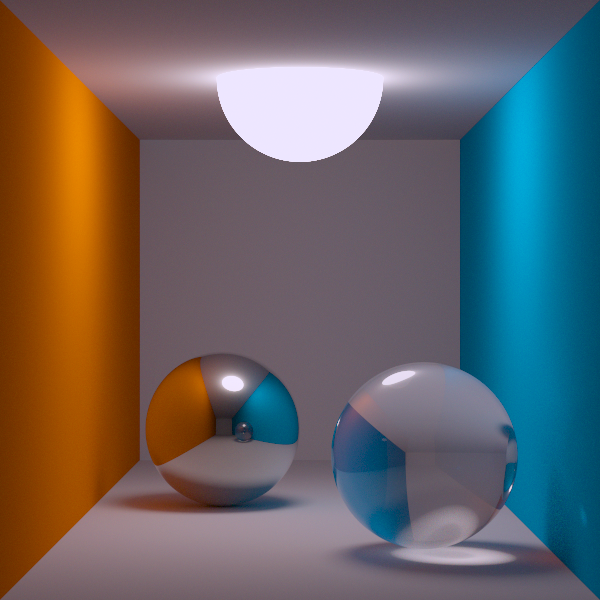
\includegraphics[width=0.45\textwidth]{images/Path_Tracing_High}

\end{frame}


\end{document}
